\chapter{Modern Drug Discovery Pipeline}

Drug discovery is an industrial process. From 1950 to 2008, the US Food and Drug Administration (FDA) approved 1,222 new drugs \citep{717}. In 2008 and 2009, only 21 and 24 new drugs respectively were approved for marketing in the United States \citep{716}, well below the level required to secure the future of the pharmaceutical industry, which has been struggling with decreasing approval numbers for more than a decade. This is particularly remarkable because the level of investment in pharmaceutical research and development (R\&D) has dramatically increased by 12\% on average year-on-year since 1970 and at present to about US\$50 billion per year (Figure \ref{fig:NewDrugApprovals} \citep{686}).

\begin{figure}
\centering
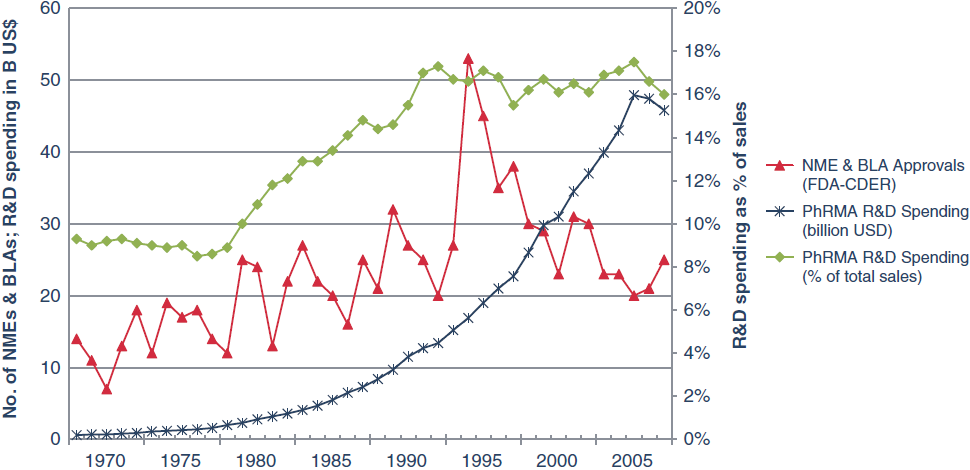
\includegraphics[width=\textwidth]{Background/NewDrugApprovals.png}
\caption{New drug approvals and R\&D investments by PhRMA-member companies from 1970 to 2009. Figure reprinted from \citep{686}.}
\label{fig:NewDrugApprovals}
\end{figure}

Drug discovery is an expensive and long-term business. A recent study in 2010 estimated that it takes US\$1.778 billion over a period of 13.5 years to develop a new drug (Figure \ref{fig:DrugDiscoveryProcess} \citep{716}). Broken down, the cost and cycle time broadly work out at US\$94 million and 1 year in hit identification, US\$166 million and 1.5 years in lead identification, US\$414 million and 2 years in lead optimization, US\$150 million and 1 year in preclinical phase, US\$273 million and 1.5 years in phase 1 clinical trials, US\$319 million and 2.5 years in phase 2 clinical trials, US\$314 million and 2.5 years in phase 3 clinical trials, and US\$48 million and 1.5 years in submission to launch.

\begin{figure}
\centering
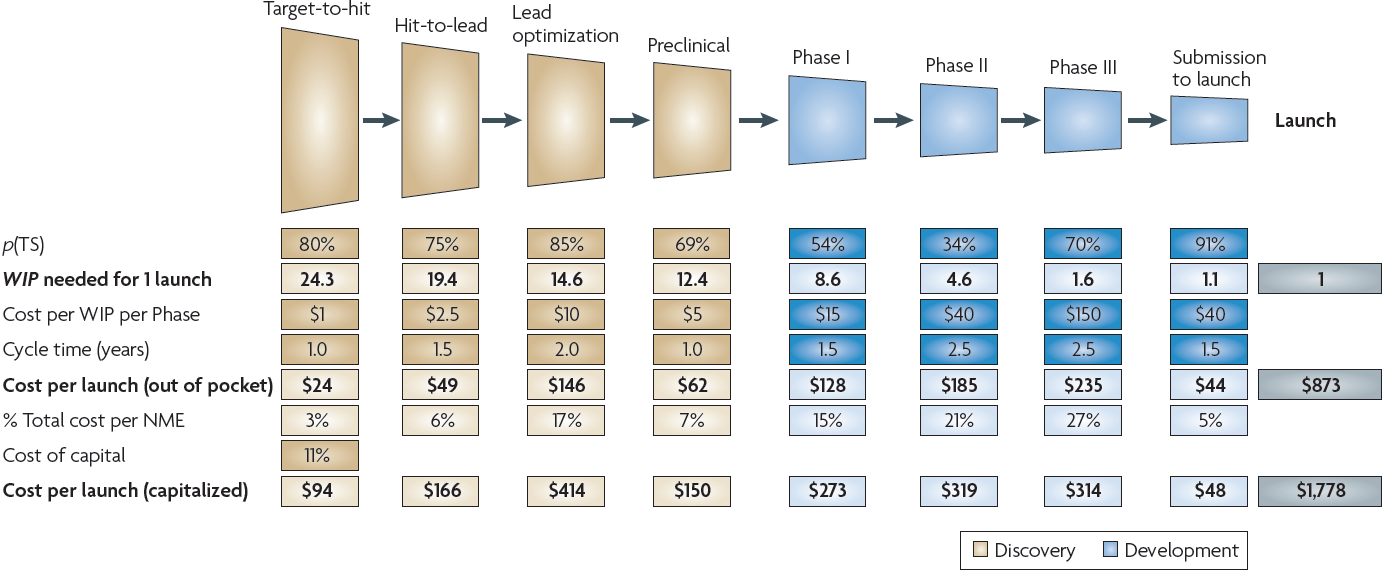
\includegraphics[width=\textwidth]{Background/DrugDiscoveryProcess.png}
\caption{R\&D model yielding costs and cycle times to successfully discover and develop a single new molecular entity (NME). Figure reprinted from \citep{716}.}
\label{fig:DrugDiscoveryProcess}
\end{figure}

Drug discovery is a high risk process and a wasteful game. It costs quite a lot to develop the ones that fail \citep{688}. It is estimated that for every 30,000 compounds synthesized, 2000 (6.7\%) enter preclinical development, 200 (0.67\%) enter phase 1 clinical trials, 40 (0.13\%) enter phase 2 clinical trials, 12 (0.04\%) enter phase 3 clinical trials, 8 (0.027\%) are approved, and 1 (0.003\%) makes a satisfactory Return On Investment (ROI) \citep{713}.

How are drugs discovered and developed? This section paints a big picture for the state-of-the-art drug discovery process, and is organized according to the note entitled ``University of Survey'' by Dr. Steve Carney, the Managing Editor of Drug Discovery Today.

Figure \ref{fig:DrugDiscoveryProcess} \citep{716} shows the common steps that underpin drug discovery, including target identification, hit identification, lead identification, lead optimization, preclinical development, and clinical trials phases 1, 2 and 3.

\section{Development of an Innovative Idea}

All projects start with an idea, whose quality ultimately determines the value of a project. An idea is initiated from either an internal experiment, an external publication, or just the leisure moment in a bar. A drug discovery idea should link a process to a fundamental pathological pathway, altering which should be expected to be curative or antisymptomatic.

\section{Establishment of a Project Team}

In order to explore the potential of an innovative idea, one needs to populate a team. A team requires individuals with different expertise. Team members are typically made up of molecular biologists, \textit{in vitro} pharmacologists, automation specialists, medicinal chemists, process chemists, toxicology specialists, \textit{in vivo} pharmacologists, pathologists, bioinformaticians, chemoinformaticians, and the like. The importance of proper planning should never be underestimated.

\section{Target Discovery}

Once a team is established, the first task is to identify a biological target \citep{706,355,356,357,797}, which is any system that can potentially be modulated by a molecule to produce a beneficial effect.

A target is generally a protein (Figure \ref{fig:USAcademicDrugDiscoveryResearchFocus} \citep{721}), although it could be from a broad spectrum of moieties, be it a molecular entity (protein, gene, miRNA, fatty acid, carbohydrate, or lipid), a disease biomarker, a biological pathway, or a crucial node on a regulatory network, as long as it is relevant to a specific disease and its progression \citep{711}.

Pharmacology is essentially the science of the interaction of components foreign to the living body with components of the living body. Such foreign compounds interact with the human body through binding to a biological target molecule. As a result, the biological function of the target is altered such that a change in a pathway is induced. It is intended that this kind of modification of the pathway will produce a beneficial effect.

\section{Hit Identification}

Once a target is selected and validated, the next task is to identify hits, which are compounds that have activity at a predetermined level against a target, but little else is known at this early stage.

Hits are usually discovered by high throughput screening \citep{795,504,736} (Figure \ref{fig:USAcademicDrugDiscoveryResearchFocus} \citep{721}), which screens hundreds of thousands or even millions of compounds against the target in a high throughput manner. For the purpose of validation, discovered hits are re-screened against an alternative assay to rule out false positives.

\begin{figure}
\centering
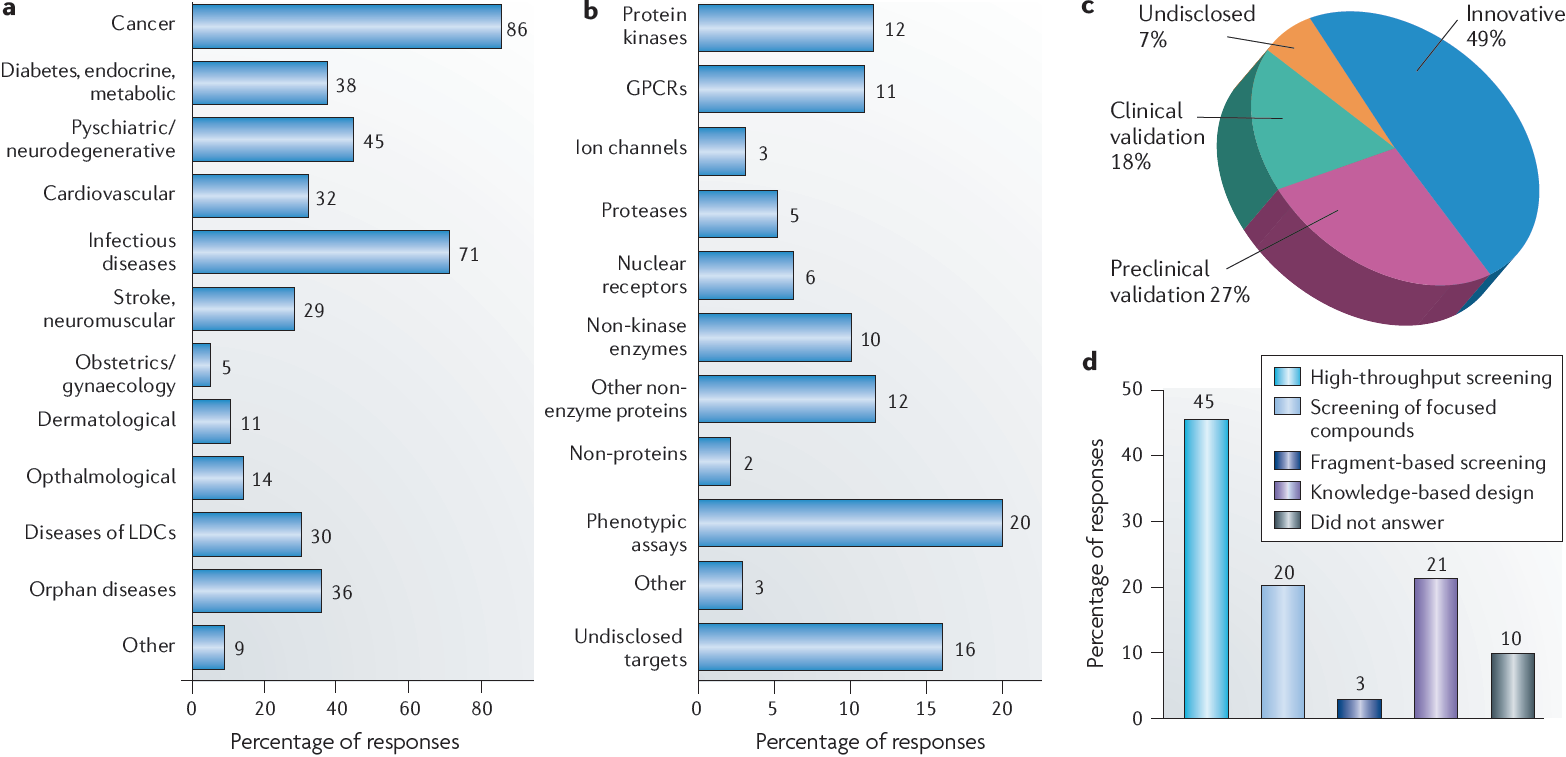
\includegraphics[width=\textwidth]{Background/USAcademicDrugDiscoveryResearchFocus.png}
\caption{Research focus of US academic and non-profit small-molecule drug discovery centres. (a) Therapeutic area. (b) Target-class focus. (c) Degree of validation of target portfolios. (d) Sources of tractable hits by discovery strategy. Figure reprinted from \citep{721}.}
\label{fig:USAcademicDrugDiscoveryResearchFocus}
\end{figure}

\section{Lead Identification}

Apart from just activity against the target, the next task is to identify those validated hits having properties that would indicate they have potential for being developed as drugs. A lead is a validated hit with several necessary properties, such as selectivity versus a panel of other targets, physicochemical characteristics, drug-like properties, and absorption, distribution, metabolism, excretion and toxicity (ADMET) properties. Only those molecules with acceptable potency, physical and ADMET properties can be advanced through lead optimization.

\section{Lead Optimization}

At this stage, medicinal chemists conduct extensive Structure-Activity Relationships (SARs) \citep{328} or use other methods \citep{661,475} to improve potency and selectivity, as well as physicochemical and drug-like properties. The optimized molecules are advanced to animal models and preliminary toxicology. They are scrutinised for potency, selectivity, bioavailability, safety, and massive productivity at a low price.

\section{Clinical Trials}

Immediately after lead optimization, the data on the successful candidates will then be submitted to the appropriate health authorities to get permission to conduct clinical investigations.

Compounds enter clinical trial at phase 1, which is focused on safety, tolerability and bioavailability rather than efficacy. The drug is administered to a small number of healthy volunteers.

Phase 2 clinical trials are focused on determining the efficacy of the drug in several hundred patients. These trials may be performed globally and give information on efficacy and allow for a further estimation of safety in a larger population.

Assuming satisfactory results from phase 2 studies, the drug will enter phase 3 clinical trials, which are in essence larger versions of the previous trials intended to answer specific questions with respect to efficacy. The trials would routinely involve several thousand patients and compare with drugs that are currently in use for the treatment of the disease. The results from these trials essentially form the basis of the risk/benefit analysis that will be submitted to the regulatory authorities.

Phase 4 clinical trials are often referred to as post-marketing studies and are performed after the medicine has been approved. These trials give a greater idea of long-term risk and benefit. The trials may involve many thousands of patients and go on for many years. Such trials may assist in indicating other uses for the medicine.

\chapterend
